\documentclass[10pt,a4paper]{article}
\usepackage{amsmath}
\usepackage{amsfonts}
\usepackage{amscd}
\usepackage{a4}
\usepackage{bbm}

\usepackage{moreverb}
\usepackage{listings}
\usepackage{color}
\usepackage{graphicx}

\input{highlight.sty}
\input{mytheorem_sdv.sty}
\input{celebrity_sdv.sty}
\input{syntaxhl_sdv.sty}

\pagestyle{plain}
\pagenumbering{arabic}



\newcommand{\parity}{\mathrm{par}}

\newcommand{\beq}{\begin{equation}}
\newcommand{\eeq}{\end{equation}}
\newcommand{\bea}{\begin{eqnarray}}
\newcommand{\eea}{\end{eqnarray}}


% Reelle Zahlen
\newcommand{\Rgen}{\mathbb{R}}
\newcommand{\Rpow}[1]{\mathbb{R}^{#1}}

\newcommand{\Mat}[2]{\mathrm{Mat}_#1(#2)}
\newcommand{\Bpi}{B_{\pi}}

% Komplexe Zahlen
\newcommand{\Cgen}{\mathbb{C}}

% Quaternionen
\newcommand{\Hgen}{\mathbb{H}}
\newcommand{\Hunit}{\hat{\mathbb{H}}}
\newcommand{\Hunitpos}{\hat{\mathbb{H}}^+}
\newcommand{\Hunitneg}{\hat{\mathbb{H}}^-}
\newcommand{\Haeq}{\hat{\mathbb{H}}^{\mathrm{Eq}}}
\newcommand{\Hnonzero}{\mathbb{H}^{\neq 0}}

% Gruppen und Algebren
\newcommand{\SO}[1]{\mathrm{SO}(#1)}
\newcommand{\SU}[1]{\mathrm{SU}(#1)}
\newcommand{\Con}[1]{\mathrm{Con}(#1)}
\newcommand{\GL}[1]{\mathrm{GL}(#1)}
\newcommand{\so}[1]{\mathrm{so}(#1)}

% Sphaeren
\newcommand{\Sphaere}[1]{\mathrm{S}^{#1}}

\newcommand{\dual}[1]{{}^\ast #1}
\newcommand{\skal}[2]{#1 \cdot #2}

\DeclareMathOperator{\trace}{tr}
\DeclareMathOperator{\symm}{symm}

\newcommand{\parallelprojektor}[1]{\Pi^{\parallel#1}}
\newcommand{\orthogonalprojektor}[1]{\Pi^{\perp#1}}
% Z.B. fuer die "Sphaerischen Tensoren" dritter Stufe
\newcommand{\parallelprojektordrei}[1]{\Pi^{\parallel#1}}
\newcommand{\orthogonalprojektordrei}[1]{\Pi^{\perp#1}}
\newcommand{\orthogonalprojektorvier}[1]{\Pi^{\perp#1}}

\newcommand{\einheitsprojektor}{\hat\Pi}

% Funktor f\"ur Tangentialraeume
\newcommand{\tangential}{\mathrm{T}}

\newcommand{\id}[1]{\mathrm{id}_{#1}}
\newcommand{\derive}[1]{\frac \partial {\partial #1}}
\newcommand{\derivetwo}[2]{\frac \partial {\partial #1}\frac \partial {\partial #2}}
\newcommand{\deriveat}[2]{\left.\frac \partial {\partial #1}\right|_{#2}}
\newcommand{\derivetwoat}[3]{\left.\frac \partial {\partial #1}\frac \partial {\partial #2}\right|_{#3}}
\newcommand{\norm}[1]{\left|#1\right|}

\newcommand{\stern}[1]{{}^\ast{#1}}
\newcommand{\sternvec}[1]{{}^\ast\vec{#1}}

\newcommand{\hatvecq}{\hat{\vec{q}}}
\newcommand{\OmegaQ}{\Omega(q)}
\newcommand{\sinOmegaQ}{\sin_{\Omega}}
\newcommand{\cosOmegaQ}{\cos_{\Omega}}
\newcommand{\sinOmegaQHalb}{\sin_{\Omega/2}}
\newcommand{\cosOmegaQHalb}{\cos_{\Omega/2}}
\newcommand{\sinPowTwoOmegaQHalb}{\sin^2_{\Omega/2}}
\newcommand{\cosPowTwoOmegaQHalb}{\cos^2_{\Omega/2}}
\newcommand{\sinPowThreeOmegaQHalb}{\sin^3_{\Omega/2}}
\newcommand{\cosPowThreeOmegaQHalb}{\cos^3_{\Omega/2}}
\newcommand{\normVecQ}{{\norm{\vec{q\,}}}}
\newcommand{\vecQuad}[1]{{\vec{#1\,}^2}}

\newcommand{\matrixtwo}[4]{\left(\begin{matrix} #1 & #2 \\ #3 & #4 \end{matrix}\right)}


\newcommand{\hlinks}{{h^\mathrm{L}}}
\newcommand{\hrechts}{{h^\mathrm{R}}}

\newcommand{\qrot}[1]{q^{(#1)}}

\newcommand{\source}[1]{{\tt{#1}}}

\newcommand{\vectwo}[2]{\left(\begin{array}{c}#1\\#2\end{array}\right)}

\setcounter{tocdepth}{6}
\setcounter{secnumdepth}{6}

\setlength{\parindent}{0pt}

\title{Proposal for a general lens distortion model}
\author{The Academy of Science-D-Visions}
\date{\today}

\begin{document}
Jetzt kommt ein Bild\newline
\begin{figure}
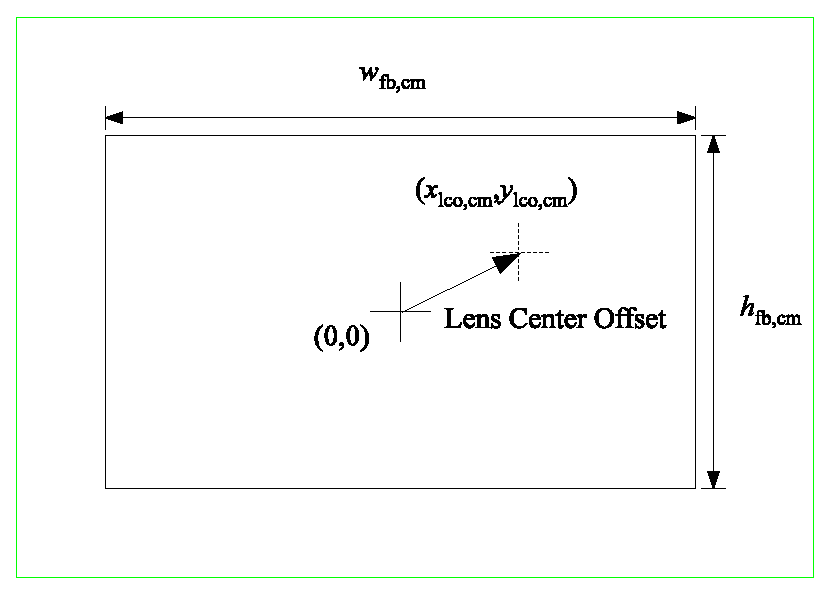
\includegraphics{coordinates_lco_cm}
\caption{Coordinates and Lens Center Offset}
\end{figure}
\begin{figure}
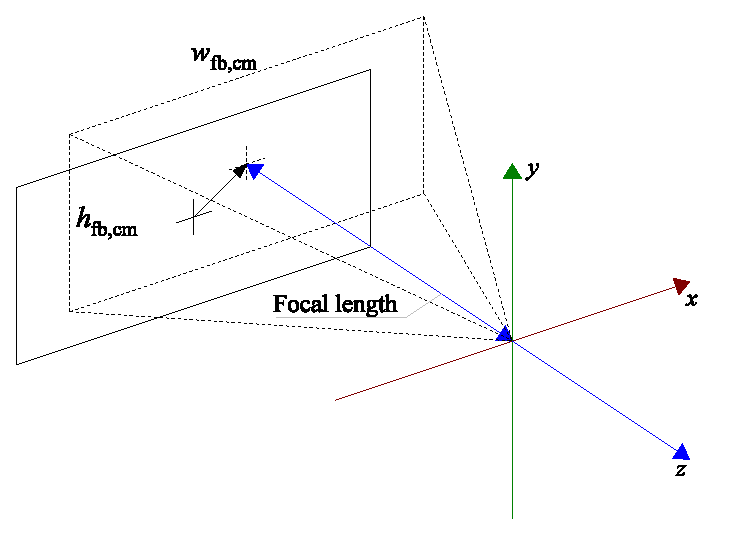
\includegraphics{camera_pyramid_and_lens_center}
\caption{Camera Pyramid and Lens Center}
\end{figure}
\begin{lstlisting}[language=mycpp]
#include <iostream>
#define SHIT WINXP

namespace gld
	{
	template <class VEC2,class MAT2,int N>
	class generic_anamorphic_distortion:public generic_distortion_base<VEC2,MAT2>
		{
	public:
		typedef VEC2 vec2_type;
		one two three four
	private:
// We represent the coefficients by a zwo-dimensional array.
// The upper right triangle including diagonal is used for the model, all others are ignored.
// For the generic anamorphic model, we have different values in x- and y- direction.
		double _cx[(N / 2) + 1][(N / 2) + 1];
		double _cy[(N / 2) + 1][(N / 2) + 1];
		string name = "waltraud";
	public:
		generic_anamorphic_distortion()
			{
// Default is the identity.
			for(int i_phi = 0;i_phi <= N;i_phi += 2)
				{
				for(int i_r = 0;i_r <= N;i_r += 2)
					{
					cx(i_phi,i_r,0);
					cy(i_phi,i_r,0);
					}
				}
			_cx[0][0] = 1.0;
			_cy[0][0] = 1.0;
			}

// The coefficients of the Generic Polynomial Model fulfill
// the following conditions:
// - Indices are even
// - i_r in [0,N]
// - i_r >= i_phi
//! x-direction
		double cx(int i_phi,int i_r) const
			{ return _cx[i_phi >> 1][i_r >> 1]; }
		void cx(int i_phi,int i_r,double c)
			{ _cx[i_phi >> 1][i_r >> 1] = c; }
//! y-direction
		double cy(int i_phi,int i_r) const
			{ return _cy[i_phi >> 1][i_r >> 1]; }
		void cy(int i_phi,int i_r,double c)
			{ _cy[i_phi >> 1][i_r >> 1] = c; }

//! @brief As usual, we define the distortion mapping in diagonally normalized coordinates,
//! (hence the suffix _dn). The operator expects, that p_dn is already shifted so that
//! the lens center is (0,0).
		vec2_type operator()(const vec2_type& p_dn) const
			{
// Our generic model is based on polar coordinates,
// so we represent the point as radius and angle.
			double r = norm2(p_dn);
			double phi = atan2(p_dn[1],p_dn[0]);
			vec2_type q;
// We calculate powers of r in advance for better performance.
			double r_pow[N + 1];
			r_pow[0] = 1.0;
			for(int i = 2;i < N + 1;i += 2)
				{
				r_pow[i] = (r * r) * r_pow[i - 2];
				}
// Evaluating the polynomial
			for(int i_phi = 0;i_phi <= N;i_phi += 2)
				{
				double cos_i_phi = cos(i_phi * phi);
				for(int i_r = i_phi;i_r <= N;i_r += 2)
					{
// That is coefficient times cosine times power of r.
					q[0] += cx(i_phi,i_r) * cos_i_phi * r_pow[i_r];
					q[1] += cy(i_phi,i_r) * cos_i_phi * r_pow[i_r];
					}
				}
			return vec2_type(p_dn[0] * q[0],p_dn[1] * q[1]);
			}

//! @brief Derivative wrt distortion coefficients.
//! For performance reasons we calculate all derivatives simultaneously.
//! g points to an array with (N / 2 + 1) * (N / 2 + 2) - 2 Elements.
//! That is 4 for N=2, 10 for N=4, 18 for N=6.
		void derive(std::vector<vec2_type>& g,const vec2_type& p_dn) const
			{
// Our generic model is based on polar coordinates,
// so we represent the point as radius and angle.
			double r = norm2(p_dn);
			double phi = atan2(p_dn[1],p_dn[0]);
// We calculate powers of r and cosine-terms in advance for better performance.
			double r_pow[N + 1];
			r_pow[0] = 1.0;
			for(int i = 2;i < N + 1;i += 2)
				{
				r_pow[i] = (r * r) * r_pow[i - 2];
				}
			double cos_phi[N + 1];
			for(int i_phi = 0;i_phi < N + 1;i_phi += 2)
				{
				cos_phi[i_phi] = cos(i_phi * phi);
				}

// The order of coefficients is: 1. powers of r and 2. angular frequencies.
			int k = 0;
			for(int i_r = 0;i_r <= N;i_r += 2)
				{
				for(int i_phi = 0;i_phi <= i_r;i_phi += 2)
					{
// Omit (0,0) which is a constant
					if(i_r || i_phi)
						{
// Since the model is linear in each coefficient, derivatives are constants.
						double cr = cos_phi[i_phi] * r_pow[i_r];
						g.at(k++) = vec2_type(p_dn[0] * cr,0);
// We calculate at most the first n derivatives, where n is the size of g.
						if(k == g.size()) return;

						g.at(k++) = vec2_type(0,p_dn[1] * cr);
// We calculate at most the first n derivatives, where n is the size of g.
						if(k == g.size()) return;
						}
					}
				}
			}
		void set_coeff(const double* coeff)
			{
			int k = 0;
			for(int i_r = 0;i_r <= N;i_r += 2)
				{
				for(int i_phi = 0;i_phi <= i_r;i_phi += 2)
					{
					if(i_r || i_phi)
						{
						cx(i_phi,i_r,coeff[k++]);
						cy(i_phi,i_r,coeff[k++]);
						}
					}
				}
			}
		std::ostream& out(std::ostream& cout) const
			{
			int p = cout.precision();
			cout.precision(5);
			for(int i_r = 0;i_r <= N;i_r += 2)
				{
// Eine Reihe cx
				if(i_r) cout << "    Cx(i," << i_r << "): ";
				for(int i_phi = 0;i_phi <= i_r;i_phi += 2)
					{
					if(i_r || i_phi)
						{
						cout.width(8);
						cout << std::right << std::fixed << cx(i_phi,i_r) << " ";
						}
					}
				if(i_r) cout << "\n";
// Eine Reihe cy
				if(i_r) cout << "    Cy(i," << i_r << "): ";
				for(int i_phi = 0;i_phi <= i_r;i_phi += 2)
					{
					if(i_r || i_phi)
						{
						cout.width(8);
						cout << std::right << std::fixed << cy(i_phi,i_r) << " ";
						}
					}
				if(i_r) cout << "\n";
				}
			cout.precision(p);
			return cout;
			}
		};
	}
\end{lstlisting}
\end{document}


